\addsec{Vorlesung 9 - Anwendungsprotokolle}

\minisec{Was bedeuten die Abkürzungen HTTP und HTML? Was ist ein 'HT' ?}
\begin{itemize}
    \item \underline{HTML:} Hypertext Markup Language
    \item \underline{HTTP:} Hypertext Transfer Protocol
    \item \underline{'HT':} Hypertext
\end{itemize}

\minisec{Erklären Sie den Zusammenhang zwischen URI, URL und URN!}
\begin{itemize}
    \item \underline{\textbf{URL: }} Spezifikation von Ort und Zugriffsmodalitäten
    \item \underline{\textbf{URL:} (\textbf{U}niform \textbf{R}esource \textbf{L}ocator)} Adressierung von Informationsobjekten mit Festlegung des Zugangs-Protokolls (Ort der Ressource). RFC2141
    \item \underline{\textbf{URN:} (\textbf{U}niform \textbf{R}esource \textbf{N}ame)} Adressierung von Objekten ohne ein Protokoll festzulegen (Eindeutige und gleichbleibende Referenz – Name der Ressource). RFC1738
    \item \textbf{URI} $=$ \textbf{URL} $\cup$ \textbf{URN}
\end{itemize}

\minisec{Wie ist ein HTTP-Request-Header aufgebaut? Wie wird der Header von den Daten getrennt, und woher weiß man die Länge der Daten?}
\begin{itemize}
    \item Aufbau:
    \begin{center}
        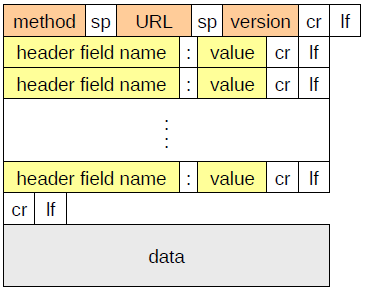
\includegraphics[width=0.5\textwidth]{img/HTTP_RequestHeader}
    \end{center}
    \item Trennung: Leerzeile
    \item Länge: Als Attribut im Header (content-length)
\end{itemize}

\minisec{Welche Gruppen von HTTP Status-Codes kennen Sie?}
\begin{itemize}
    \item 1xx – Informationen
    \item 2xx – Erfolgreiche Operation
    \item 3xx – Umleitung
    \item 4xx – Client-Fehler
    \item 5xx – Server-Fehler
    \item 9xx – Proprietäre Fehler
\end{itemize}

\minisec{Welche HTTP-Methoden existieren neben 'GET'?}
\begin{itemize}
    \item \textbf{HEAD}
    \item \textbf{POST}
    \item \textbf{PUT}
    \item \textbf{DELETE}
\end{itemize}

\minisec{Was ist MIME? Welche Attribute (mind. 3) im Header werden dazu verwendet, und was bedeuten (bzw. definieren) sie jeweils?}
\begin{itemize}
    \item \textbf{MIME} = \textbf{M}ultipurpose \textbf{I}nternet \textbf{M}ail \textbf{E}xtensions
    \item Attribute:
    \begin{itemize}
        \item \textcolor{blue}{Content-Type:} \textbf{IMAGE/JPEG}; name="picture.jpg"
        \item \textcolor{blue}{Content-Transfer-Encoding:} \textbf{BASE64}
        \item \textcolor{blue}{Content-ID:} <PINE.LNX.3.91.960212212235.325B@localhost>
    \end{itemize}
\end{itemize}

\minisec{Erklären Sie das Konzept von 'Virtual Hosts' bei HTTP!}
\begin{itemize}
    \item Auf einem Rechner sollen verschiedene Domains und Web-Server zur Verfügung stehen → Jeder Server hat die gleiche IP, aber ggf. unterschiedliche DNS-Namen!
    \item Ein oder mehrere Webserver (Software) sollen die Anfragen, für die auf dem Rechner vorhandenen Domains, beantworten
    \item Typische Anwendung: Web-Hosting (Provider)
\end{itemize}

\minisec{Wo ist der SSL-Layer im ISO/OSI oder Internet-Schichtenmodell angesiedelt?}
In der Darstellungsschicht (Schicht 6)

\minisec{Erklären Sie die Unterschiede/Vorteile/Nachteile von symmetrischer und asymmetrischer Verschlüsselung!}
\begin{itemize}
    \item Symmetrische Verschlüsselung:
    \begin{itemize}
        \item schneller
        \item braucht weniger Rechenleistung
        \item Schlüssel muss allerdings an jeden verteilt werden, der die Daten entschlüsseln muss
    \end{itemize}
    \item Asymmetrische Verschlüsselung:
    \begin{itemize}
        \item sicherer
        \item langsamer, da mehr Rechenleistung zum Entschlüsseln gebraucht wird
        \item Schlüssel müssen nicht an alle verteilt werden (private und public Key)
    \end{itemize}
\end{itemize}

\minisec{Was ist ein Zertifikat? Wer stellt es aus, und welche Informationen enthält es?}
Ein digitales Zertifikat ist ein digitaler Datensatz, der bestimmte Eigenschaften von Personen oder Objekten bestätigt und dessen Authentizität und Integrität durch kryptografische Verfahren geprüft werden kann.
Das digitale Zertifikat enthält insbesondere die zu seiner Prüfung erforderlichen Daten.
Die Ausstellung des Zertifikats erfolgt durch eine offizielle Zertifizierungsstelle, die Certification Authority (CA).

\minisec{Welche Eigenschaften hat eine Hash-Funktion? Wo wird Sie im Kontext der Verschlüsselung eingesetzt?}
\begin{itemize}
    \item \textcolor{blue}{Surjektivität} – Kein Ergebniswert (Hashwert) soll unmöglich sein, jedes Ergebnis (jeder Hashwert im definierten Wertebereich) soll tatsächlich vorkommen können.
    \item \textcolor{blue}{Effizienz} – Die Funktion muss schnell berechenbar sein, ohne großen Speicherverbrauch auskommen (der Speicherbedarf des Hashwertes soll deutlich kleiner sein als jener des Schlüssels / Eingabewertes) und sollte die Quelldaten (Eingabewerte) möglichst nur einmal lesen müssen.
    \item Hash-Funktion wird verwendet, um die private Keys zu verschlüsseln
\end{itemize}

\minisec{Wie kann man bei 2 Kommunikationspartnern ein 'Geheimnis' (z.B. einen Schlüssel zur symmetrischen Verschlüsselung) erzeugen, ohne dieses Geheimnis über das Netzwerk oder einen anderen Kanal auszutauschen?}
\medskip
\includegraphics[width=\textwidth]{img/Diffie-Hellman-Schlüsselaustausch}

\minisec{Welche Aufgaben hat das SSL Handshake Protokoll und das SSL Record Protokoll?}
\begin{itemize}
    \item \textcolor{blue}{SSL Handshake Protokoll:}
    \begin{itemize}
        \item Den stärksten gemeinsam unterstützten Algorithmus ermitteln
        \item Authentifikation der Kommunikationspartner (Client optional)
        \item Ermitteln eines Session Keys zur symmetrischen Verschlüsselung (optional)
    \end{itemize}
    \item \textcolor{blue}{SSL Record Layer:}
    \begin{itemize}
        \item Vollständig getrennt vom Handshake Protokoll
        \item Verschickt Daten symmetrisch mit dem im Handshake ausgehandelten Verschlüsselungsalgorithmen und Session Keys
        \item Bildet zu jedem Datenblock einen Message Digest zur Sicherung der Integrität
    \end{itemize}
\end{itemize}

\minisec{Warum sollte 'einfaches' FTP heute nicht mehr verwendet werden?}
Zu unsicher, Übertragung der Login-Daten als Klartext \ldots

\minisec{Warum gibt es in einem typischen Heimnetzwerk Probleme mit dem FTP 'Active' Mode?}
In Heimnetzen wird typischerweise NAT verwendet, und beim 'Active' Mode horcht der Client für die Datenverbindung auf einem zufälligen Port und teilt diesen dem Server über die Kontrollverbindung mit.
Diese Daten (IP in einem privaten Netz und Portnummer) sind aber für den NAT-Router nicht sichtbar (weil auf Anwendungsebene übertragen), und können daher vom NAT-Router nicht 'übersetzt' werden.

\minisec{Informieren Sie sich über die Entstehungsgeschichte und Funktionalität von SSL und SSH!}
\begin{itemize}
    \item \url{https://de.wikipedia.org/wiki/Secure_Shell}
    \item \url{https://de.wikipedia.org/wiki/Transport_Layer_Security}
    \item \url{https://www.kreitiv.de/ssl-tls-und-ssh-verschluesselungsprotokolle/}
\end{itemize}

\minisec{Wie funktionieren SFTP und TFTP?}
\begin{itemize}
    \item \textcolor{blue}{SFTP:} FTP über SSH Session
    \item \textcolor{blue}{TFTP:}
    \begin{itemize}
        \item sehr einfaches Protokoll für den File-Transfer
        \item die Kommunikation läuft über Port 69 und benutzt UDP, nicht TCP
        \item hat keine Authentifizierung
        \item benutzt immer 512-Byte-Blöcke
    \end{itemize}
\end{itemize}

\minisec{Welches Protokoll wird zum Versenden von Emails verwendet? Was passiert konkret bei Versenden, und wie ist das DNS beteiligt?}
\begin{itemize}
    \item Simple Mail Transfer Protokoll (SMTP)
    \item Email-Übertragung:
    \begin{enumerate}
        \item User Agent erstellt E-Mail
        \item Aufteilen der E-Mail in Header und Body
        \item Überprüfen und Zwischenspeichern der E-Mail vom Message Transfer Agent
        \item MTA sucht Mailserver des Empfängers im DNS
        \item Mail wird an Mailserver verschickt
        \item Mail wird vom Ziel-MTA überprüft
        \item Mail wird vom Empfänger Mailserver gespeichert
    \end{enumerate}
\end{itemize}

\minisec{Welche Protokolle werden zum Abrufen von Emails verwendet, und wie unterscheiden sie sich?}
\begin{itemize}
    \item \textcolor{blue}{Simple Mail Transfer Protocol (SMTP):}
    \begin{itemize}
        \item Versenden von E-Mails über TCP-Verbindung (Port 25)
        \item SMTP ist ein einfaches ASCII-Protokoll
        \item Ohne Prüfsummen, ohne Verschlüsselung
        \item Ist der Server zum Empfangen bereit, signalisiert er dies dem Client.
        Dieser sendet die Information, von wem die E-Mail kommt und wer der Empfänger ist.
        Ist der Empfänger dem Server bekannt, sendet der Client die Nachricht, der Server bestätigt den Empfang.
    \end{itemize}
    \item \textcolor{blue}{Post Office Protocol Version 3 (POP3):}
    \begin{itemize}
        \item Abholen der eMails beim Server über eine TCP-Verbindung, Port 110
        \item Befehle zum An- und Abmelden, Nachrichten herunterladen, Nachrichten auf dem Server löschen oder liegen lassen, Nachrichten ohne vorherige Übertragung vom Server direkt löschen
    \end{itemize}
    \item \textcolor{blue}{IMAP (Interactive Mail Access Protocol):}
    \begin{itemize}
        \item Hier werden die eMails nicht abgerufen und lokal gespeichert, sondern bleiben auf dem Server liegen!
    \end{itemize}
\end{itemize}

\minisec{Warum ist einfaches SMTP unsicher?}
\begin{itemize}
    \item Unverschlüsseltes, ASCII-basiertes Protokoll, Passwörter im Klartext.
    \item Einfache Möglichkeit zur Manipulation von E-Mails
\end{itemize}

\minisec{Wozu dient das (veraltete) TELNET-Protokoll? Wozu kann es (z.B. im Praktikum) sinnvoll eingesetzt werden?}
\begin{itemize}
    \item TCP ermöglicht den transparenten, interaktiven Gebrauch von „entfernten“ Maschinen
    \item verbreitetes Protokoll: TELNET, welches auf einer Client/Server-Kommunikation basiert
    \item Ein „Pseudo-Terminal“ des Servers interpretiert Zeichen, als kämen sie von der eigenen Tastatur
    \item bei Antwort des Servers umgekehrter Weg (Pseudo-Terminal fängt Antwort ab, leitet sie über TCP an den Client weiter, der die Ausgabe am Bildschirm macht
    \item \textbf{Benutzername und Passwort werden unverschlüsselt übertragen}
\end{itemize}

\minisec{Welches Protokoll sollte heute zum Login auf entfernten Rechnern verwendet werden?}
\begin{itemize}
    \item \textcolor{blue}{ssh} adressiert die Sicherheitsprobleme von telnet und rlogin.
    Es ist ein Protokoll zur Erstellung einer sicheren Verbindung zwischen zwei Systemen.
    Alle während der Verbindung gesendeten und empfangenen Daten werden mit einer 128 Bit-Verschlüsselung verschlüsselt.
    \item \textcolor{blue}{ssh} unterstützt verschiedene Authentisierungsarten:
    \begin{itemize}
        \item Bei der sogenannten hostbased-Authentifizierung akzeptiert ein Rechner ohne eigene account-spezifische Tests die Vorgaben eines fremden Rechners.
        Es wird höchstens die Identität des fremden Rechners überprüft.
        \item Die Authentifikation mit einem Passwort ist derzeit die 'übliche' Methode, um sich an einem Rechner anzumelden.
        Die Sicherheit dieses Mechanismus beruht auf der Geheimhaltung des Passwortes, dessen Übertragung allerdings verschlüsselt wird
        \item Um auch das Übertragen eines verschlüsselten Passwortes zu vermeiden, werden die sogenannten public-key-Verfahren eingesetzt
    \end{itemize}
\end{itemize}

\minisec{Wie kann mein einen sicheren 'Tunnel' zu/von einem beliebigen (TCP-) Port einrichten?}
Mit \textcolor{blue}{SSH: Port-Forwarding:}
\begin{itemize}
    \item verschlüsselte Verbindung zwischen zwei beliebigen Ports
    \item kann auch ohne Shell genutzt werden
    \item lokaler Port führt direkt auf den Zielport, als wäre dieser lokal
\end{itemize}

\minisec{Wozu wird SNMP verwendet? Welches Transportprotokoll verwendet es? Was ist ein SNMP-Agent und eine MIB?}
\begin{itemize}
    \item Transportprotokoll: UDP
    \item SNMP: Protokoll, das festlegt, wie Management-Information kommuniziert wird (Formate und Bedeutung von SNMP-Nachrichten)
    \item MIB (Management Information Base): Die MIB spezifiziert die Informationseinheiten (items), die vorgehalten werden müssen, und welche Operationen darauf erlaubt sind.
    \item SNMP wird zum Management von Geräten im Netz verwendet (Fehlerstatus etc.)
\end{itemize}